\iffalse
\let\negmedspace\undefined
\let\negthickspace\undefined
\documentclass[journal,12pt,twocolumn]{IEEEtran}
\usepackage{cite}
\usepackage{amsmath,amssymb,amsfonts,amsthm}
\usepackage{algorithmic}
\usepackage{graphicx}
\usepackage{textcomp}
\usepackage{xcolor}
\usepackage{txfonts}
\usepackage{listings}
\usepackage{enumitem}
\usepackage{mathtools}
\usepackage{gensymb}
\usepackage{comment}
\usepackage[breaklinks=true]{hyperref}
\usepackage{tkz-euclide} 
\usepackage{listings}
\usepackage{gvv}

\def\inputGnumericTable{}                                
\usepackage[latin1]{inputenc}                 
\usepackage{color}                            
\usepackage{array}                            
\usepackage{longtable}                        
\usepackage{calc}                            
\usepackage{multirow}                      
\usepackage{hhline}                           
\usepackage{ifthen}                          
\usepackage{lscape}
\usepackage{amsmath}
\newtheorem{theorem}{Theorem}[section]
\newtheorem{problem}{Problem}
\newtheorem{proposition}{Proposition}[section]
\newtheorem{lemma}{Lemma}[section]
\newtheorem{corollary}[theorem]{Corollary}
\newtheorem{example}{Example}[section]
\newtheorem{definition}[problem]{Definition}
\newcommand{\BEQA}{\begin{eqnarray}}
\newcommand{\EEQA}{\end{eqnarray}}
\newcommand{\define}{\stackrel{\triangle}{=}}
\theoremstyle{remark}
\newtheorem{rem}{Remark}


\begin{document}
%

\bibliographystyle{IEEEtran}


\vspace{3cm}

\title{
%	\logo{
Discrete 11.9.2 

\large{EE:1205 Signals and System}

Indian Institute of Technology, Hyderabad
%	}
}
\author{Prashant Maurya

EE23BTECH11218
\maketitle

\newpage

%\tableofcontents

\bigskip

\renewcommand{\thefigure}{\arabic{figure}}
\renewcommand{\thetable}{\arabic{table}}
\flushleft{\textbf{Question-2 :} Find the sum of all natural numbers lying between 100 and 1000, which are
multiples of 5.}\\
\bigskip
\textbf{Solution:}
\fi
\begin{table}[!h]
	\centering
	\begin{tabular}{|c|c|c|}
    \hline
     Parameter & Description & Value \\
    \hline
     $x(0)$ & First Term & 105\\
     \hline
     $d$ & Common Difference & 5\\
    \hline
    $n$ & Total terms & 179 \\ 
    \hline
    $x(178)$ & Last Term & 995\\
    \hline
    $m$ & No of poles & 3\\
    \hline
\end{tabular}

	\vspace{6 pt}
	\caption{Given Parameters}
\end{table}
\begin{align}
	x\brak{n}= & \brak{105+5n}\brak{u(n)}
\end{align}
On taking Z transform
\begin{align}
X\brak{z}= &\frac {x\brak{0}} {\brak{1-z^{-1}}} + \frac {dz^{-1}} {\brak{1-z^{-1}}^2} \\
= &\dfrac{105}{1-z^{-1}} + \frac{5z^{-1}}{\brak{1-z^{-1}}^{2}}\\
\implies X\brak{z}=& \dfrac{105-100z^{-1}}{{\brak{1-z^{-1}}}^2} \quad |z|>1\\
y\brak{n}=& x\brak{n}* u\brak{n}\\
\implies Y\brak{z}=& X\brak{z}U\brak{z}\\
=& \dfrac{105-100z^{-1}}{{(1-z^{-1})}^2}\frac1 {\brak{1-z^{-1}}} \\
=& \dfrac{105-100z^{-1}}{\brak{1-z^{-1}}^{3}} \quad |z|>1
\end{align}
Using contour integration to find the inverse Z-transform:\\
\begin{align}
    \implies y\brak{178}=&\dfrac{1}{2\pi j}\oint_{C}Y\brak{z} \;z^{177} \;dz\\
    =&\dfrac{1}{2\pi j}\oint_{C}\dfrac{\brak{105-100z^{-1}}{z^{177}}}{\brak{{1-z^{-1}}}^{3}} \;dz 
\end{align}
We can observe that there is only a 3 times repeated pole at $z=1$,
\begin{align}
    \implies R&=\dfrac{1}{\brak {m-1}!}\lim\limits_{z\to a}\dfrac{d^{m-1}}{dz^{m-1}}\brak {{\brak{z-a}}^{m}f\brak z}  
\end{align}
\begin{align}
    &=\dfrac{1}{\brak {2}!}\lim\limits_{z\to 1}\dfrac{d^{2}}{dz^{2}}\brak {{\brak{z-1}}^{3}\dfrac{\brak{105-100z^{-1}}z^{180}}{{\brak{z-1}}^3}}\\
    &=\dfrac{1}{2}{\lim\limits_{z\to 1}\dfrac{d^2}{dz^2}\brak{105z^{180}-100z^{179}}}\\
     &=98450
\end{align}
\begin{align}
    \therefore y\brak{178}=98450
\end{align}
\begin{figure}[ht]
    \centering
    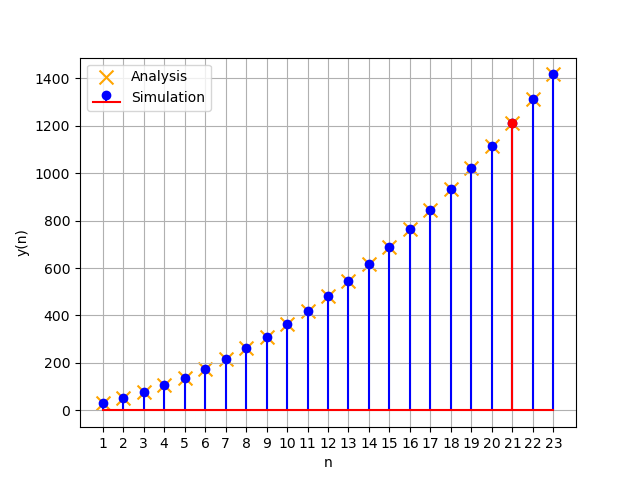
\includegraphics[width=\columnwidth]{ncert-maths/11/9/2/2/figures/fig1.png}
    \caption{Plot of $x(n)$ $vs$ $n$}
\end{figure}
%\end{document}
